
\documentclass[12pt]{article}
\usepackage[utf8]{inputenc}
\usepackage[T1]{fontenc}
\usepackage{amsmath}

\usepackage{amssymb}
\usepackage{amsmath}
%\usepackage{amsthm}
\usepackage{amsopn}
\usepackage{graphicx}
\usepackage{mathrsfs}

\usepackage{tikz}
\usetikzlibrary{fit,positioning}
\usetikzlibrary{arrows}

%\usepackage{showkeys}



%\setlength{\arraycolsep}{2pt}
%\setlength{\parskip}{.04in}
%\setlength{\footskip}{30pt}

\let\bb\mathbb       % BlackBoardBold (double letters)

\def\1{\mathbf 1}

  \def\AA{{\bb A}}\def\CC{{\bb C}}\def\DD{{\bb D}}\def\EE{{\bb E}}
  \def\GG{{\bb G}}\def\HH{{\bb H}}\def\KK{{\bb K}}\def\LL{{\bb L}}
  \def\MM{{\bb M}}\def\QQ{{\bb Q}}\def\TT{{\bb T}}\def\YY{{\bb Y}}
  \def\PP{{\bb P}}\def\II{{\bb I}}\def\WW{{\bb W}}\def\XX{{\bb X}}
  \def\VV{{\bb V}}\def\SS{{\bb S}}\def\BB{{\bb B}}\def\NN{{\bb N}}
  \def\RR{{\bb R}}\def\ZZ{{\bb Z}}\def\FF{{\bb F}}\def\DD{{\bb D}}
  \def\OO{{\bb O}}\def\JJ{{\bb J}}\def\UU{{\bb U}}

\def\cH{\mathcal H}
\def\cY{\mathcal Y}
\def\cX{\mathcal X}
\def\cA{\mathcal A}
\def\mC{\mathcal C}
\def\Ex{\mathbf E}

\def\bb{\mathbb}
%end of header
\def\hat{\widehat}
\def\bfX{\mathbf X}
\def\bfB{\mathbf B}
\def\bSigma{\boldsymbol\Sigma}
\def\bOmega{\boldsymbol\Omega}
\def\bmu{\boldsymbol\mu}
\def\bnu{\boldsymbol\nu}
\def\bPi{\boldsymbol\Pi}
\def\bX{\boldsymbol X}
\def\bx{\boldsymbol x}

\def\ci{\perp\!\!\!\perp}

\parskip=3pt
\renewcommand{\baselinestretch}{1.08}

\title{\vspace{-60pt}~\\Double sparsity in high-dimensional Gaussian mixture estimation and clustering\\Subject Overview}
\author{\vspace{-20pt}~\\ Laboratory Supervisor: A.S. Dalalyan\\
PHd Student: M. Sebbar}
\date{\today}

\begin{document}
\maketitle
\tableofcontents
\newpage
\section{Introduction}
The broad goal of this thesis is to tackle a clustering problem in the scope of mixtures model framework. More precisely, we will study the clustering of points drawn from high-dimensional Gaussian mixtures distributions.\\Thus, in the first part of this section we study the gaussian mixture model and the second part we describe the well know algorithm Expectation-Maximization (EM) and the limitations in high-dimensional setting.
\subsection{The Gaussian mixture model}

The Gaussian mixture model is an important framework where the components are Gaussian distributions with parameters $(\mu_i,\Sigma_i)$. We obtain the following distribution:
$$
p(x|\theta)=\sum_{i=1}^K\pi_i\frac{1}{(2\pi)^{d/2}|\Sigma_i|^{1/2}}\exp^{-\frac{1}{2}(x-\mu_i)^T\Sigma_i^{-1}(x-\mu_i)}=\sum_{i=1}^K\pi_i\mathcal N(x|\mu_i,\Sigma_i)
$$
with $\theta=\{\pi_1,\dots,\pi_K,\mu_1,\dots,\mu_K,\Sigma_1,\dots,\Sigma_K\}$ and $\forall i, \pi_i>0$ and $\sum_{i=1}^K=1$
\\

In the clustering problem, we would like to calculate the probability of the latent variable Z conditioned on X in order to assign X to a cluster.\\
We denote $\tau_k=P(z_k=1|x,\theta)$, from Bayes's rule we have:
$$
\tau_k=\frac{P(x|z_k=1,\theta)P(z_k=1)}{P(x)}=\frac{\pi_k \mathcal N(x|\mu_k,\Sigma_k)}{\sum_{i=1}^K\mathcal N(x|\mu_i,\Sigma_i)}
$$

where $\pi_i=P(z_i=1)$ the prior probability and $\tau_i$ the posterior.\\

We would like to estimate $\theta$ from a set of iid observations $X_1,\dots,X_N$. The related graphical model is:

%%GRAPH of pgm
\begin{figure}
\centering
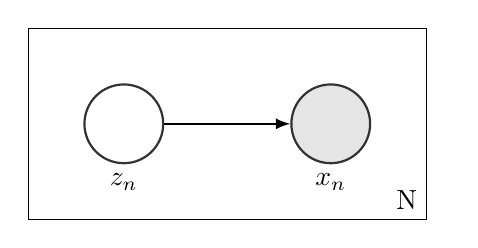
\begin{tikzpicture}
\tikzstyle{main}=[circle, minimum size = 10mm, thick, draw =black!80, node distance = 16mm]
\tikzstyle{connect}=[-latex, thick]
\tikzstyle{box}=[rectangle, draw=black!100]
  \node[main, fill = black!10] (x) [label=below:{$x_n$}] { };
  \node[main] (z) [left=of x,label=below:{$z_n$}] {};
  \path (z) edge [connect] (x);

  \node[rectangle, inner sep=7mm,draw=black!100, fit= (z) (x)] {};
\node[rectangle, below=of x, inner sep=-10mm, fit= (z) (x),label=below right:N, xshift=20mm,yshift=3mm] {};
\end{tikzpicture}
\end{figure}

The log-likelihood is:
$$
l(\theta|D)=\sum_{n=1}{N}\log{p(x_n|\theta)}
$$


Here we have the log of a sum (contrary to exponential family distribution where the log acts on a simple probability distribution) and the maximization of the log-likelihood is a non-linear problem.\\
An approach for the estimation of the maximum of log-likelihood is the Expectation-Maximization Algorithm.
\subsection{The EM Algorithm}
We will infer the values of $\{z_n\}$ conditioned to the data $\{x_n\}$. A natural approach to estimate the parameters $\theta$ is to estimate the mean of each class by deriving the log-likelihood:
$$
\hat\mu_i=\frac{\sum_{n=1}^N\tau_n^i x_n}{\sum_{n=1}^N\tau_n^i}
$$

However, as seen in ?, $\tau_n^i$ depends on the parameter estimates which depends on $\tau_n^i$. An idea would be to initialize the parameters and iterate. We calculate the posterior probability and then estimate the parameter $\theta$. This is the idea of the EM algorithm.
\\

The EM algorithm for Gaussian Mixtures would be:
\begin{enumerate}
\item[0.] Init parameters
\item Calculate (Expectation Step): $\tau_n^i(t+1)$
\item Calculate (Maximization Step):
\begin{itemize}
\item $\mu_i(t+1)=$
\item $\Sigma_i(t+1)=$
\item $\pi_i(t+1)=$
\end{itemize}
\end{enumerate}

\#Explain why complicated, pro and cons with p large


\section{A structural analysis on $\bSigma$ approach}

We consider a multivariate Gaussian distribution with mean $\bmu^*$ and covariance $\bSigma^*$ and $Y_1,\dots,Y_N \in \RR^p$ iid drawn from this distribution. We would like to estimate $\bmu^*$ and $\bSigma^*$. We know that $\hat\bmu_n=\bar Y_n$, then WLOG we consider $\mu^*=0$, the problem is to estimate $\bSigma^*$. We will study the precision matrix and consider that $\Sigma^{-1}$ is sparse. We note $\Sigma^{-1}=\Omega$.\\
If $\Sigma^{-1}_{ij}=0 \Rightarrow Y_i \ci Y_j$ conditionnaly to $Y_{l\ne\{i,j\}}$. Thus, it makes sense to impose a $L_1$ penalty on $\Sigma^{-1}$ to increase its sparsity.

\subsection{Graphical Lasso}
$$
\mathcal N(x|\mu^*,\Sigma^*)
=\frac{1}{(2\pi)^{d/2}|\Sigma^*|^{1/2}}\exp^{-\frac{1}{2}(x-\mu^*)^T\Sigma^{-1*}(x-\mu^*)}
$$
The log-likelihood, with $\mu=0$ is given by:
$$
\mathcal{L}(\Sigma)=\log\left(\prod_{n=1}^N\frac{1}{(2\pi)^{d/2}|\Sigma|^{1/2}}\exp^{-\frac{1}{2}(x_n)^T\Sigma^{-1}(x_n)}\right)
$$
\# write eqs\\
\\
$$
L(\Sigma)=C
+\frac{N}{2}\log|\Sigma^{-1}|-\frac{1}{2} tr(S_n\Sigma^{-1})
$$
Thus, considering the sparsity of $\Omega$, we impose a penalization to the maximum likelihood estimator of $\Sigma^{-1}$
$$
\hat\Omega\in argmin\left\{ \log(|\Omega|)-tr(S_n\Omega)-\lambda||\Omega||_1   \right\}
$$
A reason to use the $L_1$ penalization instead of the ridge is that for an $L_p$ penalization, the prpblem is convex for $p\geq 1$ and we have parsimonious property for $p\leq 1$.
\subsection{Column-Wise Lasso}
\section{Comments}
\section{References}

\end{document}
